% ============================================================
%  File: AppendixProbability.tex
%  \input this file as a second appendix chapter.
%  All environments reference the existing preamble.
%  British English throughout.
% ============================================================

\chapter{Probability and Statistics: A Self-Study Reference}
\label{app:prob}

Modern control systems — from Kalman filters and Linear Quadratic
Gaussian (LQG) regulators to stochastic MPC and Reinforcement Learning
(RL) — are built on probability theory.  This appendix introduces the
core ideas from scratch, assuming only basic school-level mathematics.
Every concept is illustrated with worked examples and
MATLAB code so that you can develop intuition interactively before
encountering these tools in the main text.

By the end of this appendix you should be comfortable with random
variables, Gaussian distributions, expectations, covariance matrices,
Bayes' theorem, and stochastic processes — the exact toolkit needed for
Chapters on Kalman filtering, LQG, stochastic MPC, and RL.

% =============================================================
\section{Why Probability in Control?}
\label{sec:app_prob_why}
% =============================================================

Every real control system operates in an uncertain environment.
Sensors do not report exact values — they add noise.  Actuators do not
deliver exactly the commanded force or voltage.  The plant model is
always an approximation of reality.  Disturbances (wind, load changes,
temperature) are not known in advance.

Deterministic control (classical PID, standard MPC) ignores this
uncertainty or handles it implicitly through robustness margins.
Probabilistic control treats uncertainty explicitly by modelling
unknown quantities as \emph{random variables} and designing controllers
that perform well \emph{on average} or with \emph{guaranteed
probability}.  The four main applications you will encounter in these
notes are:

\begin{itemize}[noitemsep]
  \item \textbf{Kalman filter}: optimal state estimator when process
        and measurement noise are Gaussian.
  \item \textbf{LQG control}: combines a Kalman filter with an LQR
        controller to minimise expected quadratic cost under Gaussian
        noise.
  \item \textbf{Stochastic MPC}: replaces hard constraints with
        chance constraints (e.g.\ satisfy a comfort bound with
        probability 0.95).
  \item \textbf{Reinforcement Learning}: the agent observes noisy
        states and learns an optimal policy by maximising expected
        cumulative reward.
\end{itemize}

% =============================================================
\section{Sample Spaces, Outcomes, and Events}
\label{sec:app_sample_space}
% =============================================================

\begin{defnbox}{Sample Space and Event}
The \textbf{sample space} $\Omega$ is the set of all possible outcomes
of a random experiment.  An \textbf{event} $A$ is any subset
$A \subseteq \Omega$.  The \textbf{probability} of event $A$, written
$P(A)$, is a number in $[0,1]$ that quantifies how likely $A$ is to
occur.
\end{defnbox}

\textbf{The three axioms of probability} (Kolmogorov, 1933):
\begin{enumerate}[noitemsep]
  \item $P(A) \geq 0$ for every event $A$.
  \item $P(\Omega) = 1$ (something always happens).
  \item If $A$ and $B$ are \emph{mutually exclusive} ($A \cap B = \emptyset$),
        then $P(A \cup B) = P(A) + P(B)$.
\end{enumerate}

From these three axioms every other rule of probability can be derived.
Key consequences:
\begin{itemize}[noitemsep]
  \item $P(\emptyset) = 0$
  \item $P(A^c) = 1 - P(A)$, where $A^c$ is the complement of $A$
  \item $P(A \cup B) = P(A) + P(B) - P(A \cap B)$ (inclusion--exclusion)
  \item $0 \leq P(A) \leq 1$
\end{itemize}

\begin{examplebox}{Sensor failure probability}
A temperature sensor fails independently on any given day with
probability $p = 0.02$.  Over a 5-day week, what is the probability
that it fails at least once?

\solution
Let $A_i$ be the event ``fails on day $i$''.  The complement is ``never
fails in 5 days'':
\[
  P(\text{never fails}) = (1-0.02)^5 = 0.98^5 \approx 0.904.
\]
Therefore:
\[
  P(\text{at least one failure}) = 1 - 0.904 = 0.096.
\]
There is roughly a 9.6\% chance of at least one failure per week.

\begin{lstlisting}[language=Matlab]
p_fail   = 0.02;
n_days   = 5;
p_none   = (1 - p_fail)^n_days    % 0.9039
p_atleast1 = 1 - p_none           % 0.0961
\end{lstlisting}
\end{examplebox}

% =============================================================
\section{Conditional Probability and Independence}
\label{sec:app_conditional}
% =============================================================

\begin{defnbox}{Conditional Probability}
The \textbf{conditional probability} of event $A$ given that event $B$
has occurred (with $P(B) > 0$) is:
\[
  P(A \mid B) = \frac{P(A \cap B)}{P(B)}.
\]
Intuitively, conditioning on $B$ restricts the sample space to $B$ and
rescales probabilities accordingly.
\end{defnbox}

\begin{defnbox}{Statistical Independence}
Events $A$ and $B$ are \textbf{independent} if knowing $B$ occurred
gives no information about $A$:
\[
  P(A \mid B) = P(A) \quad \Longleftrightarrow \quad
  P(A \cap B) = P(A)\,P(B).
\]
In Kalman filtering, process noise and measurement noise are assumed
to be mutually independent, which greatly simplifies the filter
equations.
\end{defnbox}

\begin{examplebox}{Conditional probability with a noisy sensor}
A room is occupied 70\% of the time.  When occupied, a motion sensor
triggers with probability 0.9.  When empty, it still triggers
(false alarm) with probability 0.05.  Given that the sensor triggered,
what is the probability the room is actually occupied?

\solution
Let $O$ = ``room occupied'', $T$ = ``sensor triggered''.
\[
  P(O) = 0.7,\quad P(T \mid O) = 0.9,\quad P(T \mid O^c) = 0.05.
\]
By the \textbf{law of total probability}:
\[
  P(T) = P(T\mid O)P(O) + P(T\mid O^c)P(O^c)
       = 0.9\times0.7 + 0.05\times0.3 = 0.645.
\]
By conditional probability:
\[
  P(O\mid T) = \frac{P(T\mid O)\,P(O)}{P(T)}
             = \frac{0.63}{0.645} \approx 0.977.
\]
If the sensor triggers, the room is occupied with about 97.7\%
confidence.

\begin{lstlisting}[language=Matlab]
P_O   = 0.7;
P_T_O = 0.9;    % true positive rate
P_T_Oc= 0.05;   % false alarm rate
P_Oc  = 1 - P_O;

P_T   = P_T_O*P_O + P_T_Oc*P_Oc;     % 0.6450
P_O_T = P_T_O * P_O / P_T             % 0.9767
\end{lstlisting}
\end{examplebox}

% =============================================================
\section{Bayes' Theorem}
\label{sec:app_bayes}
% =============================================================

\begin{defnbox}{Bayes' Theorem}
For events $A$ and $B$ with $P(B) > 0$:
\[
  {P(A \mid B) = \frac{P(B \mid A)\,P(A)}{P(B)}}.
\]
In words: the \textbf{posterior} probability of $A$ given evidence $B$
equals the \textbf{likelihood} $P(B\mid A)$ times the \textbf{prior}
$P(A)$, divided by the \textbf{marginal likelihood} (evidence) $P(B)$.
\end{defnbox}

Bayes' theorem is the mathematical foundation of the Kalman filter.
At every time step the filter:
\begin{enumerate}[noitemsep]
  \item Uses the prior state estimate (before the measurement).
  \item Updates it with the likelihood of the new measurement.
  \item Produces a posterior estimate that combines both sources of
        information optimally.
\end{enumerate}

This three-step pattern — prior $\to$ likelihood $\to$ posterior —
repeats at every time step and is precisely the \emph{predict--correct}
structure of the Kalman filter described in the main text.

\begin{notebox}{Bayes' theorem and the Kalman filter}
  The Kalman filter is the exact, closed-form solution to Bayes'
  theorem when all distributions are Gaussian and the system is
  linear.  For non-linear or non-Gaussian systems, approximate methods
  (Extended Kalman Filter, Unscented Kalman Filter, Particle Filter)
  are needed — all of which still implement the same Bayesian
  predict--correct cycle.
\end{notebox}

% =============================================================
\section{Random Variables}
\label{sec:app_rv}
% =============================================================

\begin{defnbox}{Random Variable}
A \textbf{random variable} (RV) $X$ is a function that assigns a
numerical value to every outcome in the sample space $\Omega$.  It
is \textbf{discrete} if it takes countably many values and
\textbf{continuous} if it takes values in a continuous range.
\end{defnbox}

\subsection{Discrete Random Variables}
\label{subsec:app_discrete}

A discrete RV is characterised by its
\textbf{probability mass function} (PMF):
\[
  p_X(x) = P(X = x), \qquad \sum_{\text{all }x} p_X(x) = 1.
\]

\begin{examplebox}{PMF of a discrete sensor reading}
A quantised position sensor reports integer values in
$\{-2,-1,0,1,2\}$ with equal probability.  Plot the PMF.

\solution
$p_X(x) = 1/5$ for each $x \in \{-2,-1,0,1,2\}$, zero elsewhere
(a uniform discrete distribution).

\begin{lstlisting}[language=Matlab]
x   = -2:2;
pmf = ones(1,5) / 5;

figure;
stem(x, pmf, 'filled', 'LineWidth', 1.5);
xlabel('Sensor reading x');
ylabel('P(X = x)');
title('PMF of quantised sensor');
ylim([0, 0.4]); grid on;
\end{lstlisting}

\end{examplebox}

\begin{figure}[htbp]
\centering
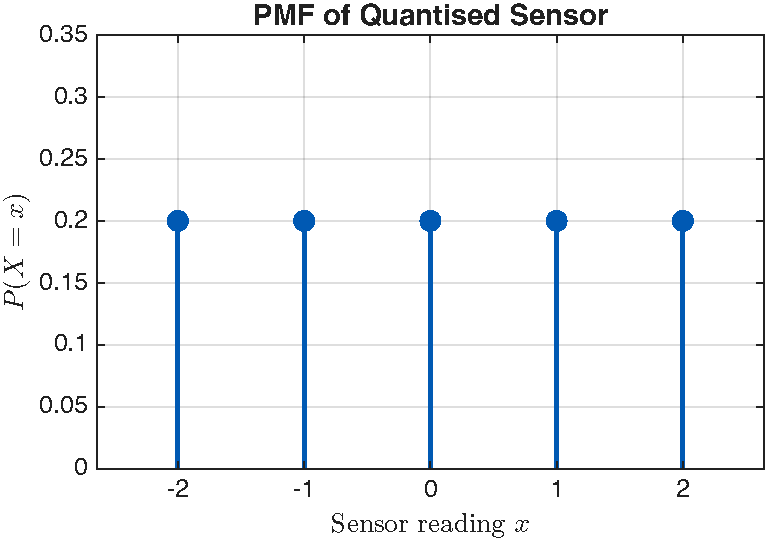
\includegraphics[width=0.65\textwidth]{Figures/fig_app_pmf_discrete.pdf}
\caption{PMF of the quantised sensor.  Each of the five possible readings has equal probability $1/5$.}
\label{fig:app_pmf_discrete}
\end{figure}

\subsection{Continuous Random Variables}
\label{subsec:app_continuous}

A continuous RV is characterised by its
\textbf{probability density function} (PDF) $f_X(x)$, defined so that:
\[
  P(a \leq X \leq b) = \int_a^b f_X(x)\,\mathrm{d}x,
  \qquad
  \int_{-\infty}^{\infty} f_X(x)\,\mathrm{d}x = 1.
\]

\begin{alertbox}{PDF values are NOT probabilities}
  $f_X(x)$ can exceed 1.  Only \emph{areas} under the PDF curve
  represent probabilities.  $P(X = x) = 0$ for any single point $x$
  (a continuous RV never takes an exact value).
\end{alertbox}

The \textbf{cumulative distribution function} (CDF) collects
probability up to $x$:
\[
  F_X(x) = P(X \leq x) = \int_{-\infty}^{x} f_X(t)\,\mathrm{d}t.
\]

% =============================================================
\section{Key Probability Distributions}
\label{sec:app_distributions}
% =============================================================

\subsection{Uniform Distribution}
\label{subsec:app_uniform}

\begin{defnbox}{Uniform Distribution $\mathcal{U}(a,b)$}
$X \sim \mathcal{U}(a,b)$ has constant density on $[a,b]$:
\[
  f_X(x) = \frac{1}{b-a}, \quad a \leq x \leq b;\qquad
  f_X(x) = 0 \text{ otherwise.}
\]
Mean: $(a+b)/2$.\quad Variance: $(b-a)^2/12$.
\end{defnbox}

\subsection{The Gaussian (Normal) Distribution}
\label{subsec:app_gaussian}

The Gaussian distribution is the most important distribution in
control engineering.  Its central role follows from the
\textbf{Central Limit Theorem}: the sum of many independent random
variables tends to a Gaussian, regardless of their individual
distributions.  Sensor noise, modelling errors, and thermal
fluctuations are all well approximated as Gaussian.

\begin{defnbox}{Gaussian Distribution $\mathcal{N}(\mu, \sigma^2)$}
A scalar RV $X \sim \mathcal{N}(\mu, \sigma^2)$ has PDF:
\[
  f_X(x) = \frac{1}{\sqrt{2\pi\sigma^2}}
            \exp\!\left(-\frac{(x-\mu)^2}{2\sigma^2}\right),
  \quad x \in \mathbb{R},
\]
where $\mu$ is the \textbf{mean} (centre) and $\sigma^2$ is the
\textbf{variance} (spread).  The \textbf{standard deviation} is
$\sigma = \sqrt{\sigma^2}$.
\end{defnbox}

\begin{figure}[htbp]
\centering
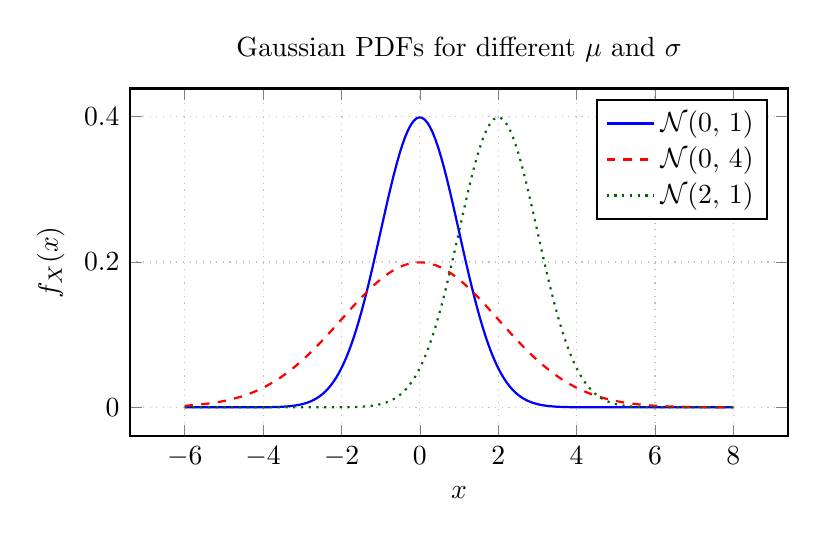
\begin{tikzpicture}
\begin{axis}[
  width=0.82\textwidth, height=6cm,
  xlabel={$x$}, ylabel={$f_X(x)$},
  title={Gaussian PDFs for different $\mu$ and $\sigma$},
  domain=-6:8, samples=200,
  legend pos=north east,
  grid=major, grid style={dotted, gray!50},
  thick
]
  \addplot[blue,  thick]{exp(-(x-0)^2/(2*1^2))/(sqrt(2*pi)*1)};
  \addlegendentry{$\mathcal{N}(0,\,1)$}

  \addplot[red,   thick, dashed]{exp(-(x-0)^2/(2*2^2))/(sqrt(2*pi)*2)};
  \addlegendentry{$\mathcal{N}(0,\,4)$}

  \addplot[black!60!green, thick, dotted]
          {exp(-(x-2)^2/(2*1^2))/(sqrt(2*pi)*1)};
  \addlegendentry{$\mathcal{N}(2,\,1)$}
\end{axis}
\end{tikzpicture}
\caption{Gaussian PDFs.  Increasing $\sigma^2$ widens the bell curve
  (more uncertainty); shifting $\mu$ moves its centre (different
  expected value).}
\label{fig:gauss_pdf}
\end{figure}

\textbf{The 68--95--99.7 rule} (essential for engineering):
\[
  P(\mu - \sigma \leq X \leq \mu + \sigma)    \approx 0.683,\quad
  P(\mu - 2\sigma \leq X \leq \mu + 2\sigma)  \approx 0.954,\quad
  P(\mu - 3\sigma \leq X \leq \mu + 3\sigma)  \approx 0.997.
\]

\begin{examplebox}{Gaussian sensor noise in MATLAB}
A temperature sensor measures a true value of $20\,^\circ$C with
additive Gaussian noise of standard deviation $\sigma = 0.5\,^\circ$C.
Simulate 10\,000 measurements and verify the 68--95--99.7 rule.

\begin{lstlisting}[language=Matlab]
mu    = 20;
sigma = 0.5;
N     = 10000;
rng(42);               % fix random seed for reproducibility

meas  = mu + sigma * randn(1, N);

% Verify 68-95-99.7 rule
in1sig = mean(abs(meas - mu) <= 1*sigma)   % ~0.683
in2sig = mean(abs(meas - mu) <= 2*sigma)   % ~0.954
in3sig = mean(abs(meas - mu) <= 3*sigma)   % ~0.997

% Plot histogram vs true PDF
figure;
histogram(meas, 60, 'Normalization', 'pdf', ...
          'FaceColor', [0.6 0.8 1], 'EdgeColor', 'none');
hold on;
x_range = linspace(17, 23, 300);
pdf_true = normpdf(x_range, mu, sigma);
plot(x_range, pdf_true, 'r-', 'LineWidth', 2);
xlabel('Measurement (deg C)');
ylabel('Probability density');
title('Simulated Gaussian sensor noise');
legend('Histogram','True PDF'); grid on;
\end{lstlisting}

\solution
Running the code confirms all three percentages to within 1\% of
their theoretical values.  \texttt{normpdf(x,mu,sigma)} evaluates the
Gaussian PDF; \texttt{normcdf} evaluates the CDF.

\end{examplebox}

\begin{figure}[htbp]
\centering
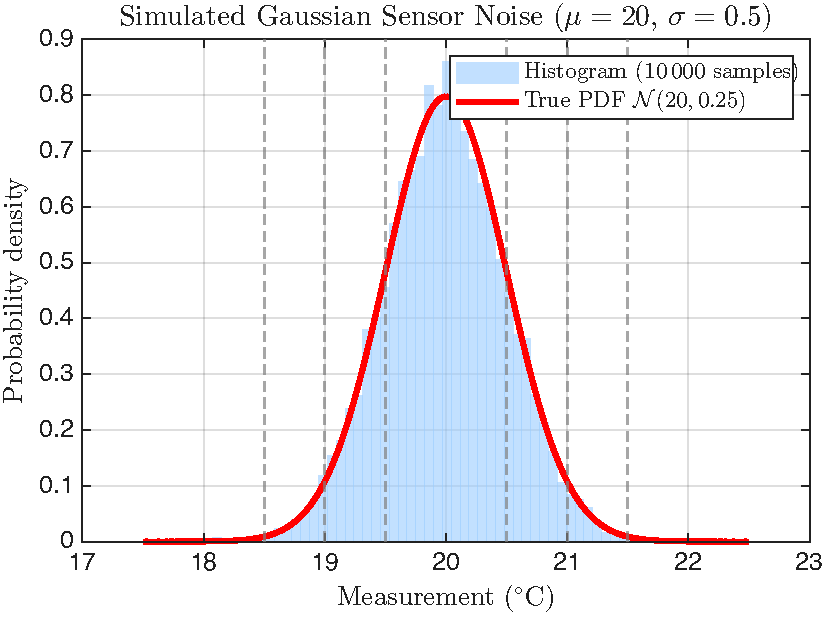
\includegraphics[width=0.72\textwidth]{Figures/fig_app_gauss_hist.pdf}
\caption{Histogram of 10\,000 simulated sensor measurements overlaid with the true Gaussian PDF $\mathcal{N}(20,\,0.25)$.  Dashed lines mark $\pm 1\sigma$, $\pm 2\sigma$, and $\pm 3\sigma$ bounds.}
\label{fig:app_gauss_hist}
\end{figure}

\subsection{Exponential and Other Useful Distributions}

\begin{center}
\renewcommand{\arraystretch}{1.3}
\begin{tabular}{>{\bfseries\sffamily\small}l >{\small}l >{\small}l >{\small}l}
\toprule
Distribution & PDF / PMF & Mean & Variance \\
\midrule
Uniform $\mathcal{U}(a,b)$ &
  $\tfrac{1}{b-a}$ &
  $\tfrac{a+b}{2}$ &
  $\tfrac{(b-a)^2}{12}$ \\
Gaussian $\mathcal{N}(\mu,\sigma^2)$ &
  $\tfrac{1}{\sqrt{2\pi\sigma^2}}e^{-(x-\mu)^2/2\sigma^2}$ &
  $\mu$ & $\sigma^2$ \\
Exponential $\mathrm{Exp}(\lambda)$ &
  $\lambda e^{-\lambda x}$, $x\geq0$ &
  $1/\lambda$ & $1/\lambda^2$ \\
Bernoulli $\mathrm{Bern}(p)$ &
  $p^x(1-p)^{1-x}$, $x\in\{0,1\}$ &
  $p$ & $p(1-p)$ \\
Poisson $\mathrm{Poi}(\lambda)$ &
  $e^{-\lambda}\lambda^k/k!$, $k=0,1,\ldots$ &
  $\lambda$ & $\lambda$ \\
\bottomrule
\end{tabular}
\end{center}

% =============================================================
\section{Expectation, Variance, and Standard Deviation}
\label{sec:app_moments}
% =============================================================

\begin{defnbox}{Expected Value (Mean)}
The \textbf{expected value} (or \textbf{mean}) of a random variable
$X$ is its probability-weighted average:
\[
  \mu = \mathbb{E}[X] =
  \begin{cases}
    \displaystyle\sum_x x\,p_X(x) & \text{(discrete)}, \\[6pt]
    \displaystyle\int_{-\infty}^{\infty} x\,f_X(x)\,\mathrm{d}x &
    \text{(continuous)}.
  \end{cases}
\]
\end{defnbox}

\begin{defnbox}{Variance and Standard Deviation}
The \textbf{variance} measures the average squared deviation from the
mean:
\[
  \sigma^2 = \mathrm{Var}(X) = \mathbb{E}\!\left[(X-\mu)^2\right]
           = \mathbb{E}[X^2] - \mu^2.
\]
The \textbf{standard deviation} $\sigma = \sqrt{\mathrm{Var}(X)}$ has
the same units as $X$ and is the most intuitive measure of spread.
\end{defnbox}

\textbf{Linearity of expectation} (always true, regardless of
dependence):
\[
  \mathbb{E}[aX + bY + c] = a\,\mathbb{E}[X] + b\,\mathbb{E}[Y] + c.
\]

\textbf{Variance under linear transformation:}
\[
  \mathrm{Var}(aX + b) = a^2\,\mathrm{Var}(X).
\]

\begin{examplebox}{Mean and variance of measurement noise}
The measurement noise in a Kalman filter is modelled as
$v_k \sim \mathcal{N}(0, R)$ with $R = 0.25$.  What fraction of
measurements lie within $\pm 1\,^\circ$C of the true value?

\solution
$\sigma = \sqrt{0.25} = 0.5$.  We need
$P(-1 \leq v_k \leq 1) = P(-2\sigma \leq v_k \leq 2\sigma) \approx
0.954$.

\begin{lstlisting}[language=Matlab]
R     = 0.25;
sigma = sqrt(R);        % 0.5

% Probability within +/- 1 degree
prob = normcdf(1, 0, sigma) - normcdf(-1, 0, sigma)  % 0.9545

% Alternatively, using the standard normal
z = 1 / sigma;          % 2 standard deviations
prob2 = 2*normcdf(z) - 1                             % 0.9545

% Mean and variance via Monte Carlo
v = sigma * randn(1, 1e6);
fprintf('Sample mean:     %.4f\n', mean(v))    % ~0
fprintf('Sample variance: %.4f\n', var(v))     % ~0.25
\end{lstlisting}
\end{examplebox}

% =============================================================
\section{Covariance and Correlation}
\label{sec:app_covariance}
% =============================================================

\begin{defnbox}{Covariance}
The \textbf{covariance} of two random variables $X$ and $Y$ measures
how they vary together:
\[
  \mathrm{Cov}(X,Y) = \mathbb{E}\!\left[(X - \mathbb{E}[X])
                       (Y - \mathbb{E}[Y])\right]
                     = \mathbb{E}[XY] - \mathbb{E}[X]\,\mathbb{E}[Y].
\]
Note that $\mathrm{Cov}(X,X) = \mathrm{Var}(X)$.  If $X$ and $Y$ are
independent, $\mathrm{Cov}(X,Y) = 0$ (but the converse is not
generally true).
\end{defnbox}

\begin{defnbox}{Pearson Correlation Coefficient}
The \textbf{correlation coefficient} normalises covariance to the
range $[-1,1]$:
\[
  \rho_{XY} = \frac{\mathrm{Cov}(X,Y)}{\sigma_X \sigma_Y}.
\]
$\rho = 1$: perfect positive linear relationship; $\rho = -1$:
perfect negative; $\rho = 0$: uncorrelated (no linear relationship).
\end{defnbox}

\begin{examplebox}{Covariance and correlation in MATLAB}
\begin{lstlisting}[language=Matlab]
rng(0);
N  = 1000;
x  = randn(N,1);
y1 = 2*x + 0.5*randn(N,1);   % highly correlated with x
y2 = randn(N,1);               % independent of x

% Covariance matrices
C1 = cov(x, y1)    % large off-diagonal entries
C2 = cov(x, y2)    % near-zero off-diagonal

% Correlation coefficients
rho1 = corr(x, y1)   % close to +1
rho2 = corr(x, y2)   % close to  0

% Scatter plots
figure;
subplot(1,2,1); scatter(x, y1, 5, '.'); grid on;
xlabel('x'); ylabel('y_1'); title(sprintf('\\rho = %.2f', rho1));
subplot(1,2,2); scatter(x, y2, 5, 'r.'); grid on;
xlabel('x'); ylabel('y_2'); title(sprintf('\\rho = %.2f', rho2));
\end{lstlisting}

\end{examplebox}

\begin{figure}[htbp]
\centering
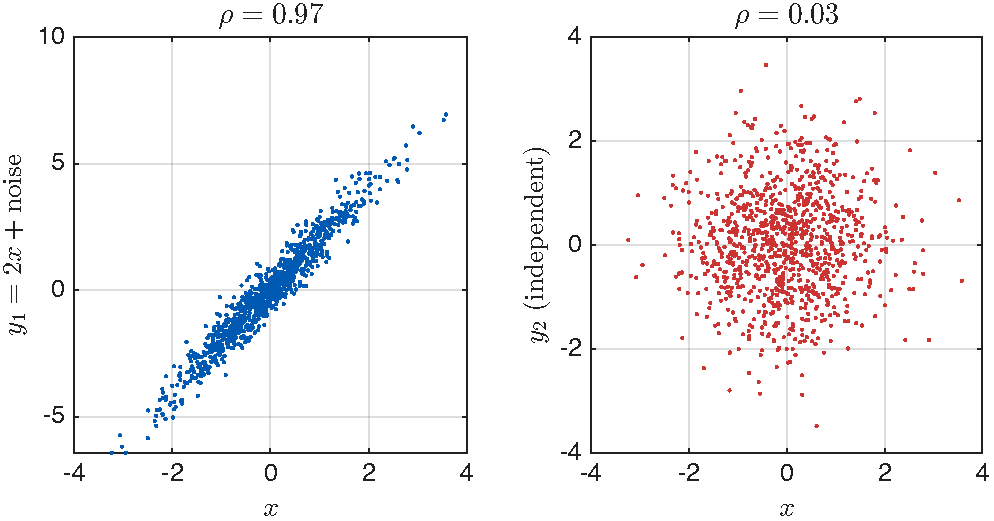
\includegraphics[width=0.85\textwidth]{Figures/fig_app_covariance_scatter.pdf}
\caption{Scatter plots illustrating correlation.  Left: $y_1 = 2x + \text{noise}$ shows strong positive correlation ($\rho \approx 0.97$).  Right: $y_2$ is independent of $x$ ($\rho \approx 0$).}
\label{fig:app_covariance_scatter}
\end{figure}

% =============================================================
\section{The Multivariate Gaussian Distribution}
\label{sec:app_mvgauss}
% =============================================================

State vectors in control systems are multi-dimensional.  The Kalman
filter propagates a full \emph{joint} probability distribution over all
state components simultaneously, which requires the multivariate
generalisation of the Gaussian.

\begin{defnbox}{Multivariate Gaussian $\mathcal{N}(\boldsymbol{\mu}, \Sigma)$}
A random vector $x \in \mathbb{R}^n$ follows a
\textbf{multivariate Gaussian} distribution with mean vector
$\boldsymbol{\mu} \in \mathbb{R}^n$ and
\textbf{covariance matrix} $\Sigma \in \mathbb{R}^{n\times n}$ if its
PDF is:
\[
  f(x) = \frac{1}{(2\pi)^{n/2}\sqrt{\det(\Sigma)}}
                  \exp\!\left(-\frac{1}{2}
                  (x-\boldsymbol{\mu})^\top
                  \Sigma^{-1}
                  (x-\boldsymbol{\mu})\right).
\]
The covariance matrix $\Sigma$ must be \textbf{symmetric positive
semi-definite}: $\Sigma = \Sigma^\top$ and $\Sigma \succeq 0$.
\end{defnbox}

The diagonal entries of $\Sigma$ are the individual variances:
$\Sigma_{ii} = \mathrm{Var}(x_i)$.  The off-diagonal entries are
covariances: $\Sigma_{ij} = \mathrm{Cov}(x_i, x_j)$.

\begin{figure}[htbp]
\centering
\begin{tikzpicture}
\begin{axis}[
  width=0.78\textwidth, height=6.5cm,
  title={Contours of bivariate Gaussian PDFs},
  xlabel={$x_1$}, ylabel={$x_2$},
  xmin=-4, xmax=4, ymin=-4, ymax=4,
  axis equal,
  grid=major, grid style={dotted, gray!50},
  legend pos=outer north east,
  legend style={font=\small}
]
  % Uncorrelated: contours are circles
  \foreach \r in {0.5, 1.0, 1.5, 2.0}{
    \addplot[blue, thick, domain=0:360, samples=100]
        ({\r*cos(x)}, {\r*sin(x)});
  }
  \addlegendentry{$\Sigma=I$ (uncorrelated)}

  % Correlated: contours are tilted ellipses
  % Sigma = [1 0.8; 0.8 1], eigendecomp gives tilt
  \foreach \r in {0.5, 1.0, 1.5, 2.0}{
    \addplot[red, dashed, thick, domain=0:360, samples=120]
        ({0.949*\r*cos(x) + 0.316*\r*sin(x)},
         {0.949*\r*cos(x) - 0.316*\r*sin(x)});
  }
  \addlegendentry{$\Sigma=\begin{bmatrix}1&0.8\\0.8&1\end{bmatrix}$}
\end{axis}
\end{tikzpicture}
\caption{Equal-probability contours of two bivariate Gaussian
  distributions.  When $\Sigma = I$ the contours are circles
  (independent components).  When off-diagonal covariance is large the
  contours tilt into ellipses aligned with the correlated direction.}
\label{fig:bivariate_gauss}
\end{figure}

\begin{notebox}{Covariance matrices in the Kalman filter}
  The Kalman filter maintains the state estimate as
  $x_k \sim \mathcal{N}(\hat{x}_k, P_k)$,
  where $P_k$ is the \textbf{error covariance matrix}.  At each step:
  \begin{itemize}[noitemsep]
    \item \textbf{Prediction}: $P$ grows (uncertainty increases
          because the model is imperfect).
    \item \textbf{Correction}: $P$ shrinks (the measurement reduces
          uncertainty).
  \end{itemize}
  The Kalman gain $K$ is precisely the factor that balances how much
  to trust the model prediction versus the new measurement.
\end{notebox}

\begin{examplebox}{Multivariate Gaussian samples in MATLAB}
Generate samples from a bivariate Gaussian with
$\boldsymbol{\mu} = [1,\;-2]^\top$ and
$\Sigma = \begin{bmatrix} 2 & 0.8 \\ 0.8 & 1 \end{bmatrix}$.

\begin{lstlisting}[language=Matlab]
mu    = [1; -2];
Sigma = [2, 0.8; 0.8, 1];

% Check Sigma is positive definite
eig(Sigma)           % both positive: [0.4781; 2.5219]

% Draw 2000 samples
rng(1);
N       = 2000;
samples = mvnrnd(mu', Sigma, N);  % N x 2 matrix

% Plot
figure;
scatter(samples(:,1), samples(:,2), 8, '.', ...
        'MarkerEdgeColor', [0.2 0.4 0.8]);
hold on;
plot(mu(1), mu(2), 'r+', 'MarkerSize', 15, 'LineWidth', 2);
xlabel('x_1'); ylabel('x_2');
title('Samples from \mathcal{N}(\mu, \Sigma)');
legend('Samples','Mean'); grid on; axis equal;

% Verify sample statistics
fprintf('Sample mean:  [%.3f, %.3f]\n', mean(samples));
disp('Sample covariance:'); disp(cov(samples))
\end{lstlisting}

\end{examplebox}

\begin{figure}[htbp]
\centering
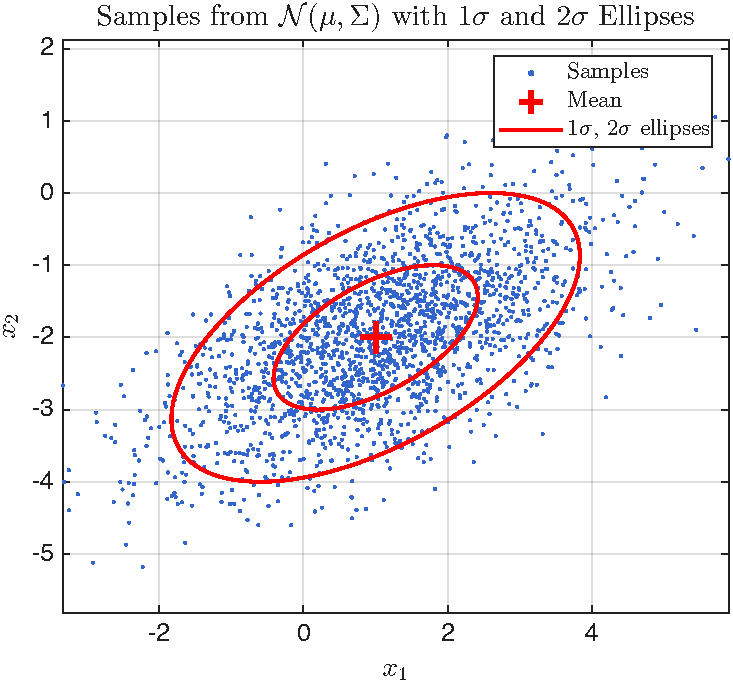
\includegraphics[width=0.65\textwidth]{Figures/fig_app_mvnrnd_samples.pdf}
\caption{2\,000 samples from a bivariate Gaussian with $\boldsymbol{\mu} = [1,\,-2]^\top$ and correlated covariance.  Red ellipses show the $1\sigma$ and $2\sigma$ contours, which are tilted due to the positive off-diagonal covariance.}
\label{fig:app_mvnrnd_samples}
\end{figure}

% =============================================================
\section{Conditional Multivariate Gaussian}
\label{sec:app_cond_gauss}
% =============================================================

A second closure property of Gaussians---equally important as linear transformations---is that \emph{conditioning} a joint Gaussian on some of its components produces another Gaussian. This is the mathematical foundation of both the Kalman filter update step and Gaussian process regression (Chapter~11).

\begin{defnbox}{Conditional Gaussian Distribution}
Suppose $\begin{bmatrix} x_a \\ x_b \end{bmatrix} \sim \mathcal{N}\!\left(\begin{bmatrix} \mu_a \\ \mu_b \end{bmatrix},\; \begin{bmatrix} \Sigma_{aa} & \Sigma_{ab} \\ \Sigma_{ba} & \Sigma_{bb} \end{bmatrix}\right)$.
Then the conditional distribution of $x_a$ given $x_b = \bar{x}_b$ is:
\[
	x_a \mid x_b = \bar{x}_b \;\sim\; \mathcal{N}\!\bigl(\mu_{a|b},\; \Sigma_{a|b}\bigr)
\]
where:
\begin{align*}
	\mu_{a|b} &= \mu_a + \Sigma_{ab}\,\Sigma_{bb}^{-1}\,(\bar{x}_b - \mu_b) \\
	\Sigma_{a|b} &= \Sigma_{aa} - \Sigma_{ab}\,\Sigma_{bb}^{-1}\,\Sigma_{ba}
\end{align*}
\end{defnbox}

Two observations are worth noting:
\begin{itemize}[noitemsep]
	\item The conditional mean $\mu_{a|b}$ is the prior mean $\mu_a$ plus a correction proportional to how far the observed value $\bar{x}_b$ deviates from its prior mean $\mu_b$. The matrix $\Sigma_{ab}\,\Sigma_{bb}^{-1}$ determines how much $x_a$ adjusts in response --- this is exactly the structure of the Kalman gain.
	\item The conditional covariance $\Sigma_{a|b}$ does not depend on the observed value $\bar{x}_b$; it depends only on the prior covariance structure. Observing $x_b$ always reduces variance by the same amount, regardless of what value is observed.
\end{itemize}

\begin{examplebox}{Conditional Gaussian: numerical example}
Let $\begin{bmatrix} x_1 \\ x_2 \end{bmatrix} \sim \mathcal{N}\!\left(\begin{bmatrix} 0 \\ 0 \end{bmatrix},\; \begin{bmatrix} 1 & 0.8 \\ 0.8 & 1 \end{bmatrix}\right)$. Compute $x_1 \mid x_2 = 1.5$.

\solution
Identify $\mu_a = 0$, $\mu_b = 0$, $\Sigma_{aa} = 1$, $\Sigma_{ab} = 0.8$, $\Sigma_{bb} = 1$. Then:
\begin{align*}
	\mu_{1|2} &= 0 + 0.8 \cdot 1^{-1} \cdot (1.5 - 0) = 1.2 \\
	\sigma^2_{1|2} &= 1 - 0.8 \cdot 1^{-1} \cdot 0.8 = 0.36
\end{align*}
So $x_1 \mid x_2 = 1.5 \;\sim\; \mathcal{N}(1.2,\; 0.36)$. Knowing $x_2 = 1.5$ shifts our prediction of $x_1$ from~0 to~1.2, and reduces the variance from~1 to~0.36.

This is exactly how Gaussian process prediction works (Chapter~11, Section~11.2.1): the ``training outputs'' play the role of $x_b$, and the ``test output'' plays the role of $x_a$. The kernel matrix provides the covariance structure.
\end{examplebox}

% =============================================================
\section{Chance Constraints and the Inverse CDF}
\label{sec:app_chance_constraints}
% =============================================================

In stochastic MPC and GP-MPC (Chapter~11), hard state constraints $x_k \le x_{\max}$ cannot be guaranteed when the state is uncertain. Instead, we require the constraint to hold with high probability:
\[
	\Pr(x_k \le x_{\max}) \ge 1 - \delta
\]
where $\delta \in (0, 1)$ is a small violation probability (e.g.\ $\delta = 0.05$ for 95\% confidence).

If $x_k \sim \mathcal{N}(\mu_k, \sigma_k^2)$, this chance constraint can be converted to a \emph{deterministic} constraint on the mean:
\[
	\mu_k + \Phi^{-1}(1-\delta)\,\sigma_k \le x_{\max}
\]
where $\Phi^{-1}$ is the inverse CDF (quantile function) of the standard normal distribution. Common values: $\Phi^{-1}(0.95) \approx 1.645$, $\Phi^{-1}(0.975) \approx 1.960$, $\Phi^{-1}(0.99) \approx 2.326$.

The term $\Phi^{-1}(1-\delta)\,\sigma_k$ is the \emph{constraint tightening}: the safety margin grows with uncertainty $\sigma_k$ and with the required confidence level $1-\delta$. In MATLAB: \texttt{kappa = norminv(1 - delta)}.

% =============================================================
\section{Linear Transformations of Gaussian Variables}
\label{sec:app_linear_gauss}
% =============================================================

A crucial property that makes Gaussian distributions so convenient for
control is that they are \emph{closed under linear transformations}: a
linear function of a Gaussian is still Gaussian.

\begin{defnbox}{Linear Transformation of a Gaussian Vector}
If $x \sim \mathcal{N}(\boldsymbol{\mu}, \Sigma)$ and
$y = Ax + b$, then:
\[
  y \sim \mathcal{N}\!\left(
    A\boldsymbol{\mu} + b,\;
    A\Sigma A^\top
  \right).
\]
\end{defnbox}

This is exactly the \textbf{predict step} of the Kalman filter.  If
the state $x_k \sim \mathcal{N}(\hat{x}_k, P_k)$
and the system evolves as $x_{k+1} = Ax_k +
w_k$ with process noise
$w_k \sim \mathcal{N}(0, Q)$, then the predicted
state distribution is:
\[
  x_{k+1} \sim \mathcal{N}\!\left(
    A\hat{x}_k,\;
    A P_k A^\top + Q
  \right).
\]
No approximation is involved — the result is exact because all
operations are linear and all distributions are Gaussian.

\begin{examplebox}{Propagating uncertainty through a linear system}
A one-dimensional system has $x_{k+1} = 0.9\,x_k + w_k$ with
$w_k \sim \mathcal{N}(0, 0.01)$.  The initial state is
$x_0 \sim \mathcal{N}(5, 1)$.  Propagate the mean and variance for
10 steps.

\solution
At each step: $\mu_{k+1} = 0.9\,\mu_k$ and
$\sigma^2_{k+1} = 0.81\,\sigma^2_k + 0.01$.  The variance decays
towards the steady-state value
$\sigma^2_\infty = 0.01/(1-0.81) \approx 0.053$.

\begin{lstlisting}[language=Matlab]
a     = 0.9;
Q     = 0.01;    % process noise variance
mu    = 5;
P     = 1;       % initial variance
N     = 10;

mu_log = zeros(1,N+1);  P_log = zeros(1,N+1);
mu_log(1) = mu;          P_log(1) = P;

for k = 1:N
    mu = a * mu;
    P  = a^2 * P + Q;
    mu_log(k+1) = mu;
    P_log(k+1)  = P;
end

figure;
subplot(2,1,1);
plot(0:N, mu_log, 'b-o', 'LineWidth', 1.5);
ylabel('\mu_k'); title('Propagated mean'); grid on;

subplot(2,1,2);
plot(0:N, P_log, 'r-o', 'LineWidth', 1.5);
yline(Q/(1-a^2), 'k--', 'Steady state', 'LineWidth', 1);
ylabel('\sigma^2_k'); xlabel('Step k');
title('Propagated variance'); grid on;
\end{lstlisting}

\end{examplebox}

\begin{figure}[htbp]
\centering
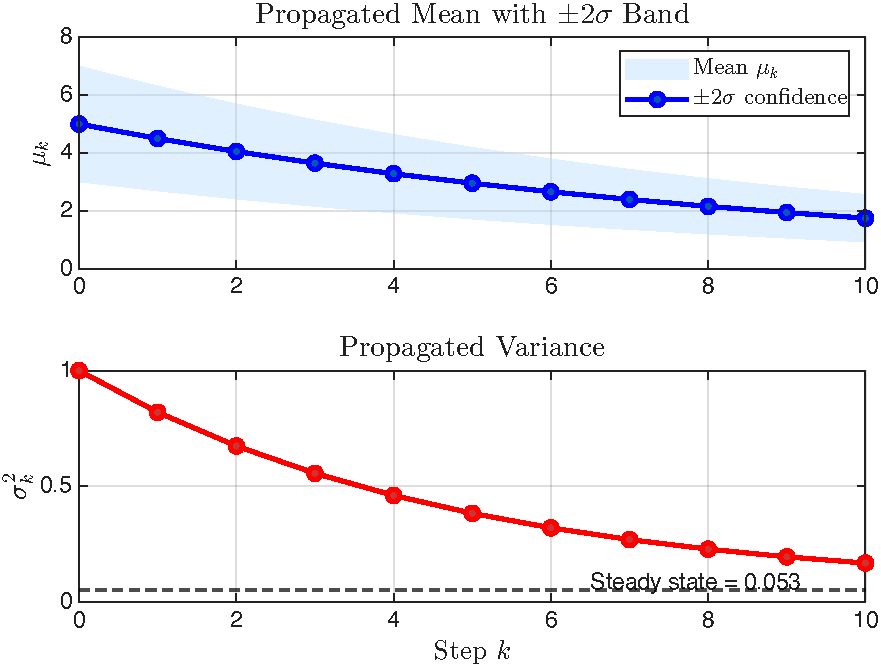
\includegraphics[width=0.75\textwidth]{Figures/fig_app_uncertainty_prop.pdf}
\caption{Propagation of a Gaussian state distribution through $x_{k+1} = 0.9\,x_k + w_k$.  Top: the mean decays towards zero with a $\pm 2\sigma$ confidence band.  Bottom: the variance converges to the steady-state value $\sigma^2_\infty = Q/(1 - a^2) \approx 0.053$.}
\label{fig:app_uncertainty_prop}
\end{figure}

% =============================================================
\section{Stochastic Processes}
\label{sec:app_stochastic}
% =============================================================

A \textbf{stochastic process} is a sequence of random variables
indexed by time: $\{X_k\}_{k=0}^{\infty}$ (discrete time) or
$\{X(t)\}_{t\geq0}$ (continuous time).  In control, the key
stochastic processes are:

\begin{itemize}[noitemsep]
  \item \textbf{White noise}: uncorrelated sequence where each sample
        is drawn independently from the same distribution.  Used to
        model process noise $w_k$ and measurement noise $v_k$ in state-space models.
  \item \textbf{Random walk}: $X_{k+1} = X_k + w_k$ where $w_k$ is
        white noise.  The variance grows without bound.
  \item \textbf{Markov process}: the future depends only on the
        present state, not the past.  State-space models are
        (first-order) Markov by construction: $x_{k+1} = f(x_k, u_k, w_k)$.
\end{itemize}

\begin{defnbox}{White Noise Assumptions in State-Space Control}
The standard Kalman filter assumptions are:
\begin{align*}
  w_k &\sim \mathcal{N}(0, Q), \quad
  \text{(process noise)} \\
  v_k &\sim \mathcal{N}(0, R), \quad
  \text{(measurement noise)} \\
  \mathbb{E}[w_k w_j^\top] &= Q\,\delta_{kj}, \quad
  \text{(uncorrelated across time)} \\
  \mathbb{E}[v_k v_j^\top] &= R\,\delta_{kj}, \quad
  \mathbb{E}[w_k v_j^\top] &= 0,
\end{align*}
where $\delta_{kj} = 1$ if $k=j$, else $0$ (Kronecker delta).
Matrices $Q \succeq 0$ and $R \succ 0$ are the noise covariance
matrices that appear explicitly in the Kalman filter equations.
\end{defnbox}

\begin{examplebox}{Simulating white noise and a random walk}
\begin{lstlisting}[language=Matlab]
N     = 200;
Q     = 0.5;      % process noise variance
rng(7);
w     = sqrt(Q) * randn(1, N);   % white noise sequence

% Verify whiteness: autocorrelation should be near zero for lag > 0
figure;
subplot(3,1,1);
plot(w); xlabel('k'); ylabel('w_k');
title('White noise sequence'); grid on;

subplot(3,1,2);
maxlag = 20;
acf = zeros(1, maxlag+1);
w_c = w - mean(w);
c0 = sum(w_c.^2);
for lag = 0:maxlag
    acf(lag+1) = sum(w_c(1:end-lag).*w_c(lag+1:end))/c0;
end
stem(0:maxlag, acf, 'filled', 'LineWidth', 1.5);
xlabel('Lag'); ylabel('ACF');
title('Autocorrelation of white noise');
yline(1.96/sqrt(N), 'r--'); yline(-1.96/sqrt(N), 'r--');

% Random walk: x_{k+1} = x_k + w_k
x = cumsum(w);
subplot(3,1,3);
plot(x, 'r'); xlabel('k'); ylabel('x_k');
title('Random walk (cumulative sum of white noise)'); grid on;
\end{lstlisting}
\solution
The autocorrelation plot confirms that white noise has zero
correlation at all non-zero lags (within statistical fluctuation).
The random walk drifts unpredictably because its variance grows as
$k \cdot Q$.

\end{examplebox}

\begin{figure}[htbp]
\centering
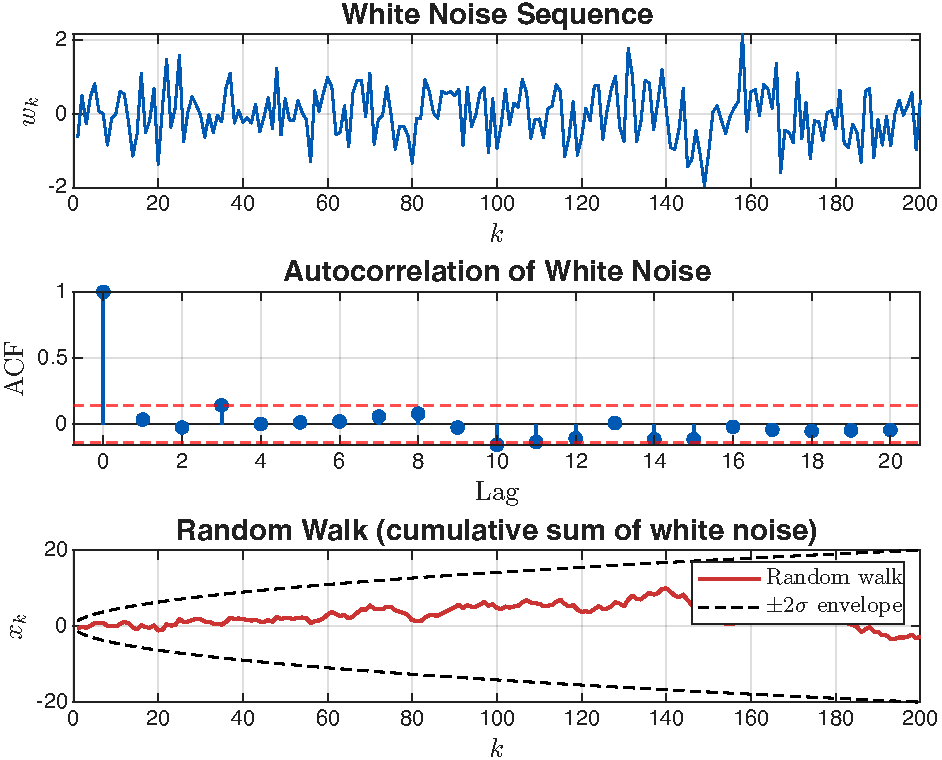
\includegraphics[width=0.82\textwidth]{Figures/fig_app_white_noise_rw.pdf}
\caption{Top: a white noise sequence $w_k \sim \mathcal{N}(0, 0.5)$.  Middle: its autocorrelation function, confirming zero correlation at all non-zero lags.  Bottom: the random walk $x_k = \sum_{i=1}^{k} w_i$ with the $\pm 2\sigma$ envelope $\pm 2\sqrt{kQ}$ showing unbounded variance growth.}
\label{fig:app_white_noise_rw}
\end{figure}

% =============================================================
\section{The Law of Large Numbers and the Central Limit Theorem}
\label{sec:app_lln_clt}
% =============================================================

These two theorems are the bedrock of statistical intuition.

\begin{defnbox}{Law of Large Numbers (LLN)}
Let $X_1, X_2, \ldots, X_N$ be independent, identically distributed
(i.i.d.) random variables with mean $\mu$.  The sample mean converges
to the true mean as the sample size grows:
\[
  \bar{X}_N = \frac{1}{N}\sum_{i=1}^N X_i \;\xrightarrow{\;N\to\infty\;}\; \mu.
\]
\end{defnbox}

\begin{defnbox}{Central Limit Theorem (CLT)}
Under the same conditions (i.i.d., finite variance $\sigma^2$), the
\emph{standardised} sample mean converges in distribution to a
standard Gaussian:
\[
  \frac{\bar{X}_N - \mu}{\sigma/\sqrt{N}}
  \;\xrightarrow{\;d\;}\;
  \mathcal{N}(0,1)
  \quad \text{as } N \to \infty.
\]
This is why Gaussian noise is such a universal model: it emerges
naturally as the aggregate effect of many small, independent
perturbations.
\end{defnbox}

\begin{examplebox}{Demonstrating the CLT in MATLAB}
Show that the sample mean of $N$ uniform random variables approaches
a Gaussian as $N$ increases.

\begin{lstlisting}[language=Matlab]
n_trials = 5000;
figure;

for idx = 1:4
    N = 10^idx;                          % N = 10, 100, 1000, 10000
    % Sum N uniform[0,1] samples, then standardise
    raw  = rand(n_trials, N);
    xbar = mean(raw, 2);                 % n_trials x 1 sample means
    mu_u = 0.5;  sig_u = 1/sqrt(12*N);  % theoretical mean and std
    z    = (xbar - mu_u) / sig_u;

    subplot(2,2,idx);
    histogram(z, 40, 'Normalization','pdf', ...
              'FaceColor',[0.6 0.8 1], 'EdgeColor','none');
    hold on;
    x_range = linspace(-4, 4, 200);
    plot(x_range, normpdf(x_range), 'r-', 'LineWidth', 2);
    title(sprintf('N = %d', N));
    xlabel('z'); ylabel('PDF'); grid on;
    xlim([-4 4]);
end
sgtitle('Central Limit Theorem: convergence to Gaussian');
\end{lstlisting}
\solution
Even for $N=10$ the histogram already resembles a bell curve.  By
$N=1000$ the agreement with the standard Gaussian (red curve) is
almost perfect.

\end{examplebox}

\begin{figure}[htbp]
\centering
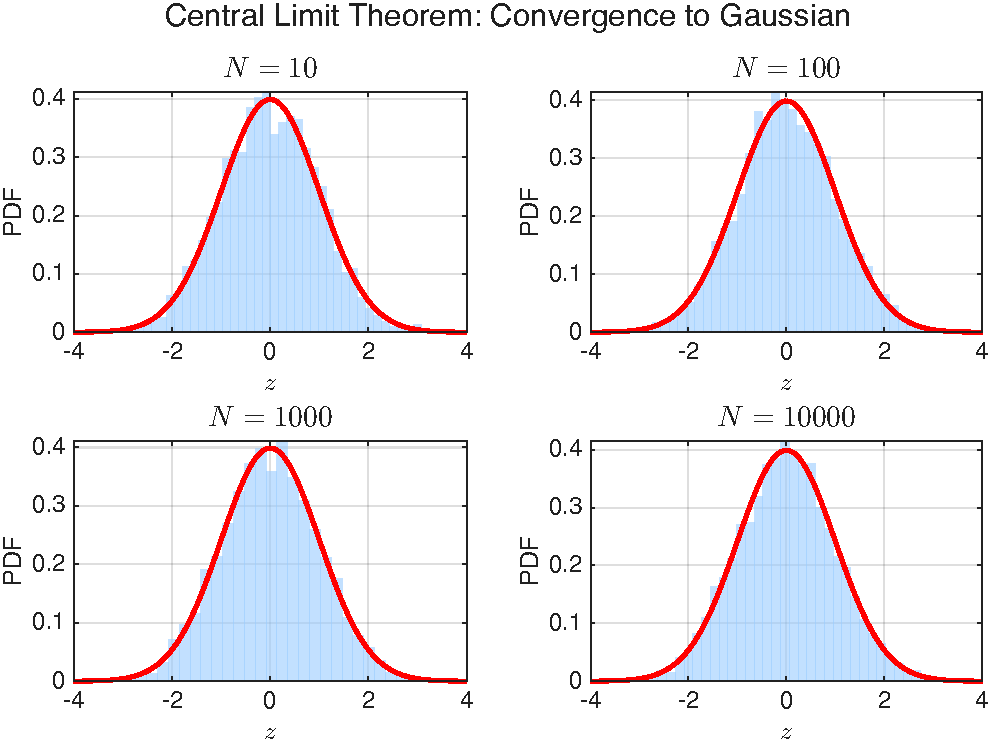
\includegraphics[width=0.82\textwidth]{Figures/fig_app_clt_demo.pdf}
\caption{Central Limit Theorem in action.  The standardised sample mean of $N$ uniform random variables (blue histogram) converges to the standard Gaussian (red curve) as $N$ increases.}
\label{fig:app_clt_demo}
\end{figure}

% =============================================================
\section{Monte Carlo Methods}
\label{sec:app_montecarlo}
% =============================================================

Monte Carlo methods approximate expectations and probabilities by
drawing many random samples.  They are used in stochastic MPC to
evaluate chance constraints (e.g.\ ``what fraction of scenarios
violate a temperature bound?'') and in RL to estimate policy value
functions.

\begin{defnbox}{Monte Carlo Estimation}
To estimate $\mathbb{E}[g(X)]$ for some function $g$ and random
variable $X$:
\begin{enumerate}[noitemsep]
  \item Draw $N$ i.i.d.\ samples $x^{(1)}, x^{(2)}, \ldots, x^{(N)}$
        from the distribution of $X$.
  \item Compute the sample average:
        $\hat{\mathbb{E}}[g(X)] = \dfrac{1}{N}\sum_{i=1}^N g(x^{(i)})$.
\end{enumerate}
By the LLN this estimate converges to the true expectation.  The
standard error of the estimate is $\sigma_{g(X)}/\sqrt{N}$, so
accuracy improves as $1/\sqrt{N}$.
\end{defnbox}

\begin{examplebox}{Monte Carlo chance constraint evaluation}
In a stochastic MPC application, room temperature at the next step is
$x_1 \sim \mathcal{N}(21.5,\; 0.04)$ (mean 21.5$^\circ$C, variance
0.04).  Estimate the probability that the comfort constraint
$x_1 \geq 21\,^\circ$C is satisfied.

\begin{lstlisting}[language=Matlab]
mu_x  = 21.5;
var_x = 0.04;
N     = 100000;
rng(3);
x_samples = mu_x + sqrt(var_x) * randn(1, N);

% Monte Carlo probability estimate
p_mc      = mean(x_samples >= 21)     % ~0.9938

% Exact answer via CDF
p_exact   = 1 - normcdf(21, mu_x, sqrt(var_x))  % 0.9938

fprintf('Monte Carlo: %.4f\n', p_mc);
fprintf('Exact:       %.4f\n', p_exact);
\end{lstlisting}
\solution
Both methods give $P(x_1 \geq 21) \approx 0.9938$, i.e.\ the
comfort constraint is satisfied 99.4\% of the time.  In stochastic
MPC this would be expressed as the chance constraint
$P(x_1 \geq 21) \geq 0.95$.

\end{examplebox}

\begin{figure}[htbp]
\centering
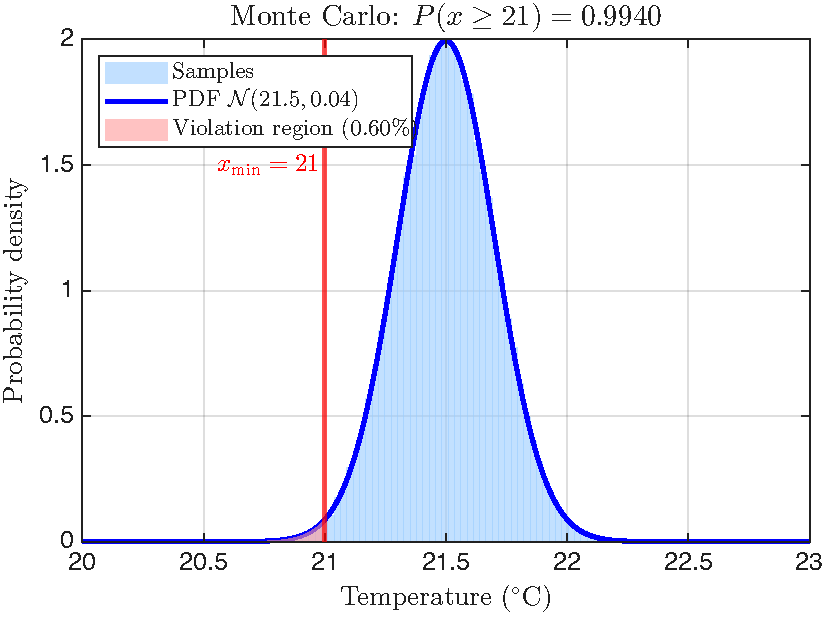
\includegraphics[width=0.72\textwidth]{Figures/fig_app_monte_carlo.pdf}
\caption{Monte Carlo evaluation of the chance constraint $P(x \geq 21) \geq 0.95$.  The shaded red region to the left of $x_{\min} = 21$ is the constraint violation area, which contains only $\approx 0.6\%$ of the probability mass.}
\label{fig:app_monte_carlo}
\end{figure}

% =============================================================
\section{Connecting Probability to the Kalman Filter}
\label{sec:app_kalman_prob}
% =============================================================

With the tools of this appendix, the Kalman filter equations can now
be understood probabilistically rather than just algorithmically.

The \textbf{state-space model} is:
\begin{align}
  {x}_{k+1} &= A{x}_k + B{u}_k + {w}_k,
  \qquad {w}_k \sim \mathcal{N}({0}, Q), \label{eq:ss1}\\
  {y}_k     &= C{x}_k + {v}_k,
  \qquad {v}_k \sim \mathcal{N}({0}, R). \label{eq:ss2}
\end{align}

The Kalman filter maintains a Gaussian belief over the state:
\[
  p({x}_k \mid {y}_{0:k}) = \mathcal{N}(\hat{{x}}_k, P_k).
\]

\textbf{Predict step} (propagate using the system model):
\begin{align}
  \hat{{x}}_{k|k-1} &= A\hat{{x}}_{k-1} + B{u}_{k-1}, \\
  P_{k|k-1}                 &= A P_{k-1} A^\top + Q.
\end{align}
This is the linear transformation rule from
Section~\ref{sec:app_linear_gauss}.

\textbf{Correct step} (update using the new measurement):
\begin{align}
  K_k               &= P_{k|k-1} C^\top
                        (C P_{k|k-1} C^\top + R)^{-1},
                        \quad\text{(Kalman gain)} \\
  \hat{{x}}_k &= \hat{{x}}_{k|k-1}
                        + K_k({y}_k - C\hat{{x}}_{k|k-1}), \\
  P_k               &= (I - K_k C)\,P_{k|k-1}.
\end{align}
The Kalman gain $K_k$ is the optimal Bayesian weighting between the
model prediction and the measurement.  When $R$ is large (noisy
sensor), $K_k \to 0$ and the filter trusts the model.  When $Q$ is
large (uncertain model), $K_k$ increases and the filter trusts the
measurement.

\begin{examplebox}{One-dimensional Kalman filter in MATLAB}
Estimate the position of a slowly drifting signal with process noise
$Q = 0.1$ and measurement noise $R = 2$.

\begin{lstlisting}[language=Matlab]
A = 1;  C = 1;  Q = 0.1;  R = 2;
N = 60;  rng(5);

% Simulate true state and measurements
x_true = cumsum([10, sqrt(Q)*randn(1,N-1)]);
y_meas = x_true + sqrt(R)*randn(1,N);

% Kalman filter
x_hat = zeros(1,N);  P = 10;  x_est = 10;

for k = 1:N
    % Predict
    x_pred = A * x_est;
    P_pred = A^2 * P + Q;

    % Correct
    K      = P_pred * C / (C^2 * P_pred + R);
    x_est  = x_pred + K * (y_meas(k) - C*x_pred);
    P      = (1 - K*C) * P_pred;
    x_hat(k) = x_est;
end

% Plot
figure;
plot(x_true, 'k-',  'LineWidth', 1.5); hold on;
plot(y_meas, 'b.',  'MarkerSize', 8);
plot(x_hat,  'r-',  'LineWidth', 2);
legend('True state','Measurements','Kalman estimate');
xlabel('Time step k'); ylabel('Position');
title('1-D Kalman Filter'); grid on;
\end{lstlisting}
\solution
The Kalman estimate (red) tracks the true state (black) much more
closely than the raw noisy measurements (blue dots), demonstrating the
filter's noise-rejection capability.

\end{examplebox}

\begin{figure}[htbp]
\centering
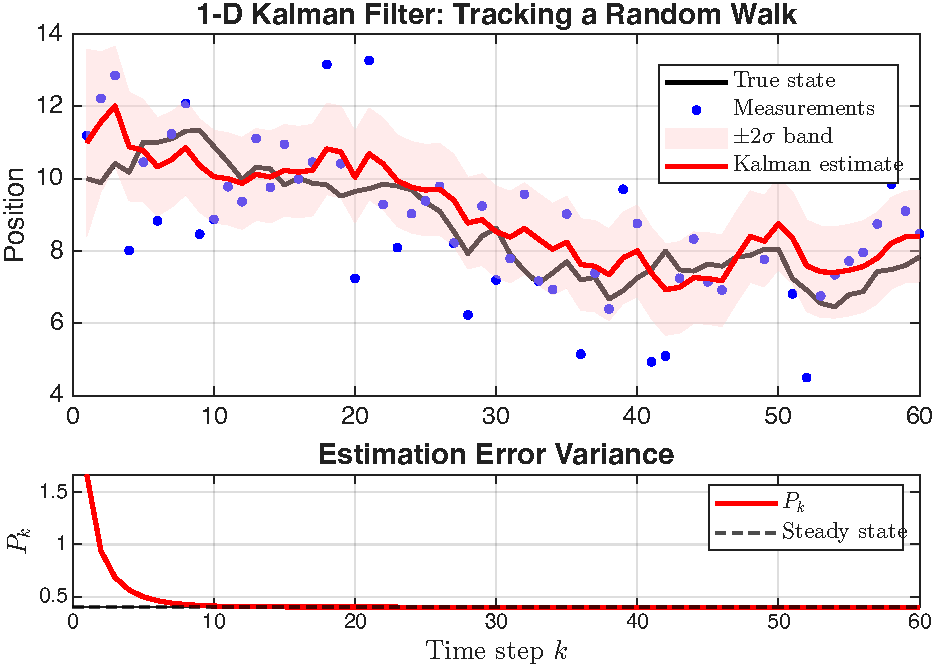
\includegraphics[width=0.82\textwidth]{Figures/fig_app_kalman_1d.pdf}
\caption{1-D Kalman filter tracking a random walk.  Top: the Kalman estimate (red) tracks the true state (black) far more closely than the noisy measurements (blue dots); the shaded band shows $\pm 2\sigma$ confidence.  Bottom: the estimation error variance $P_k$ converges quickly to its steady-state value.}
\label{fig:app_kalman_1d}
\end{figure}

% =============================================================
\section{Probability in Reinforcement Learning}
\label{sec:app_rl_prob}
% =============================================================

Reinforcement Learning frames the control problem as a
\textbf{Markov Decision Process} (MDP), which is a direct application
of the probabilistic tools developed in this appendix.

\begin{defnbox}{Markov Decision Process}
An MDP is defined by the tuple $(\mathcal{S}, \mathcal{A},
\mathcal{P}, r, \gamma)$:
\begin{itemize}[noitemsep]
  \item $\mathcal{S}$: state space (e.g.\ room temperatures)
  \item $\mathcal{A}$: action space (e.g.\ heater power levels)
  \item $\mathcal{P}(s' \mid s, a)$: \textbf{transition probability} —
        probability of reaching state $s'$ from state $s$ under action
        $a$
  \item $r(s,a)$: reward function (e.g.\ negative energy cost)
  \item $\gamma \in [0,1)$: discount factor for future rewards
\end{itemize}
The agent's goal is to find a policy $\pi(a \mid s)$ (a conditional
probability distribution over actions given states) that maximises
the \textbf{expected discounted return}:
\[
  J(\pi) = \mathbb{E}_\pi\!\left[\sum_{k=0}^{\infty} \gamma^k r(s_k, a_k)\right].
\]
\end{defnbox}

Every concept used in this definition — conditional probability,
expectation, Markov property — has been covered in the earlier sections
of this appendix.  The connection between RL and MPC is that both seek
to maximise a sum of future rewards/costs; RL does so by
\emph{learning} the optimal policy from data rather than by solving an
explicit optimisation problem at each step.

% =============================================================
\section{Quick Reference: MATLAB Commands for Probability}
\label{sec:app_prob_ref}
% =============================================================

\begin{center}
\renewcommand{\arraystretch}{1.35}
\begin{tabular}{>{\ttfamily\small}l >{\small}l >{\small}l}
\toprule
\normalfont\textbf{MATLAB command} & \textbf{Operation} &
\textbf{Notes} \\
\midrule
randn(m,n)           & Standard Gaussian samples     & $\mathcal{N}(0,1)$, size $m\times n$ \\
rand(m,n)            & Uniform $[0,1]$ samples       & Size $m\times n$ \\
rng(seed)            & Set random seed               & For reproducibility \\
normpdf(x,mu,sig)    & Gaussian PDF                  & Scalar or vector $x$ \\
normcdf(x,mu,sig)    & Gaussian CDF                  & $P(X\leq x)$ \\
norminv(p,mu,sig)    & Inverse CDF (quantile)        & $x$ such that $P(X\leq x)=p$ \\
mvnrnd(mu,Sigma,N)   & Multivariate Gaussian samples & $N$ rows \\
mvnpdf(X,mu,Sigma)   & Multivariate Gaussian PDF     & \\
mean(x)              & Sample mean                   & Along first non-singleton dim \\
var(x)               & Sample variance               & Unbiased ($N-1$ denominator) \\
std(x)               & Sample standard deviation     & $\sqrt{\texttt{var}(x)}$ \\
cov(X)               & Sample covariance matrix      & \texttt{X} is $N\times p$ data matrix \\
corr(x,y)            & Pearson correlation            & Returns scalar in $[-1,1]$ \\
autocorr(x,n)        & Sample autocorrelation         & Up to lag $n$ \\
histogram(x,k)       & Histogram                     & Use \texttt{'Normalization','pdf'} \\
eig(Sigma)           & Eigenvalues of $\Sigma$        & Check positive definiteness \\
chol(Sigma)          & Cholesky factorisation         & For sampling multivariate Gaussian \\
\bottomrule
\end{tabular}
\end{center}

\begin{summarybox}{Probability Summary for Control Engineers}
\begin{enumerate}[noitemsep]
  \item \textbf{Everything uncertain is a random variable.}  Sensor
        noise, model errors, and disturbances are all modelled as
        random variables with known distributions.
  \item \textbf{The Gaussian is central.}  Sensor noise and process
        disturbances are almost always modelled as Gaussian because of
        the CLT, and because Gaussians are closed under linear
        transformations.
  \item \textbf{Mean and covariance matrix} fully characterise a
        Gaussian distribution.  The Kalman filter propagates exactly
        these two quantities.
  \item \textbf{Bayes' theorem is the theoretical backbone} of all
        state estimation.  The Kalman filter is its exact solution
        under linearity and Gaussianity.
  \item \textbf{$Q$ and $R$ are design choices.}  The process noise
        covariance $Q$ and measurement noise covariance $R$ in the
        Kalman filter determine how much the filter trusts the model
        versus the sensor.  Larger $R$ $\Rightarrow$ trust the model
        more; larger $Q$ $\Rightarrow$ trust the sensor more.
  \item \textbf{Chance constraints in stochastic MPC} replace hard
        bounds with probabilistic ones:
        $P(Cx_k \leq d) \geq 1-\epsilon$.  Monte Carlo or analytical
        Gaussian CDF methods evaluate these constraints.
  \item \textbf{RL uses expectations everywhere.}  Value functions,
        policy gradients, and Bellman equations are all defined in
        terms of expected rewards under a probability distribution over
        future trajectories.
\end{enumerate}
\end{summarybox}

